\documentclass{article}
\usepackage{amsmath}
\usepackage{tikz}
\usetikzlibrary{patterns}

\begin{document}

The allowed region of integer solutions for the exponents \( v_0 \) and \( \bar{v}_0 \) in the ansatz for the \((m_1,m_2,m_3)=(m,m,0)\) amplitudes in equation \eqref{eq:m00ansatz}.

\begin{center}
    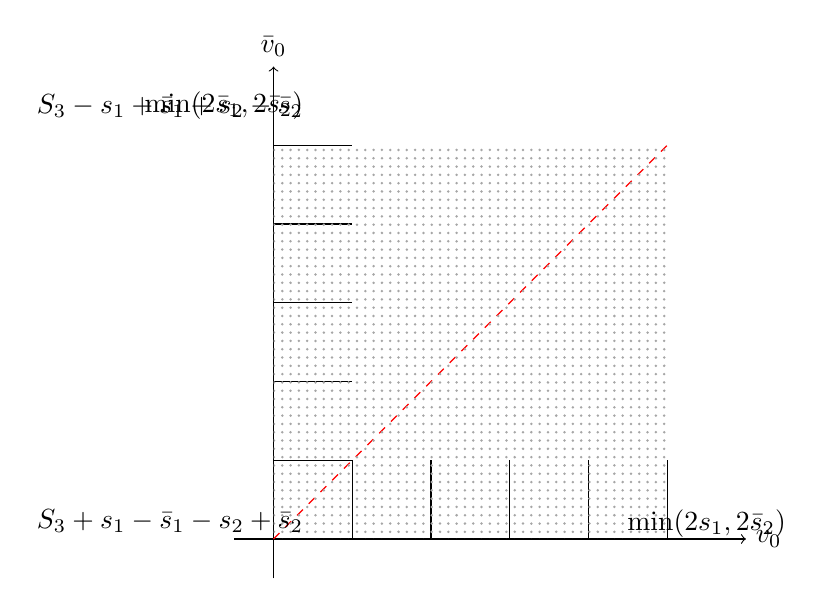
\begin{tikzpicture}[scale=1]
        % Axes
        \draw[->] (-0.5,0) -- (6,0) node[right] {$v_0$};
        \draw[->] (0,-0.5) -- (0,6) node[above] {$\bar{v}_0$};

        % Grid lines
        \foreach \x in {0,...,5}
            \draw (\x,0) -- (\x,1);
        \foreach \y in {0,...,5}
            \draw (0,\y) -- (1,\y);

        % Dashed line
        \draw[dashed, color=red] (0,0) -- (5,5);

        % Patterns
        \fill[pattern=dots, pattern color=gray!70] (0,0) rectangle (5,5);

        % Labels
        \node at (0.5, 5.5) [left] {\(\min(2\bar{s}_1, 2\bar{s}_2)\)};
        \node at (5.5, 0.5) [below] {\(\min(2s_1, 2\bar{s}_2)\)};
        \node at (0.5, 0.5) [below left] {\(S_3 + s_1 - \bar{s}_1 - s_2 + \bar{s}_2\)};
        \node at (0.5, 5.5) [left] {\(S_3 - s_1 + \bar{s}_1 + s_2 - \bar{s}_2\)};
    \end{tikzpicture}
\end{center}

\end{document}